
In this chapter, the mathematical description of the multi-scale model and its discretization is presented. 
We use the multi-scale chemo-electro-mechanical model that was introduced in literature \cite{Roehrle2012,Heidlauf2013,Heidlauf2015Diss,Mordhorst2015}. Additional models known from literature are incorporated that  were previously only simulated in isolation: The multidomain description for electrophysiology \cite{Klotz2020}, a model of neural stimulation \cite{Cisi2008} and sensory organ models such as the muscle spindle model of Mileusnic et al. \cite{Mileusnic2006Spindle}. Similarly, models of Golgi tendon organs can be added \cite{Mileusnic2006Golgi}.

% components of the multi-scale model
\begin{figure}%
  \centering%
  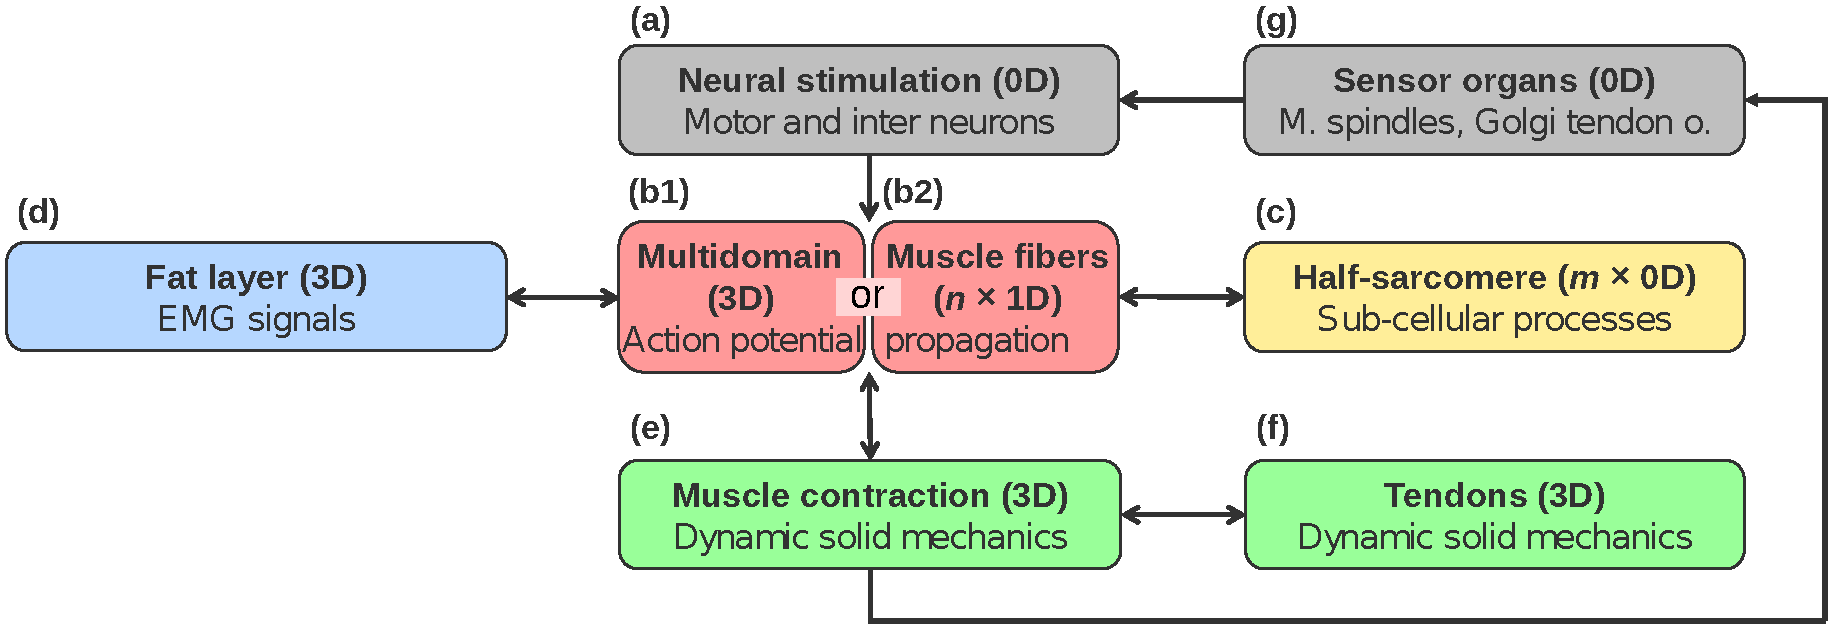
\includegraphics[width=\textwidth]{images/theory/model_schematic.pdf}%
  \caption{Interacting components of the multi-scale model.}%
  \label{fig:multi-scale-model}%
\end{figure}

\Cref{fig:multi-scale-model} shows an overview of the components of the implemented multi-scale model.
A pool of motor neurons drives the stimulation of the muscular system in \cref{fig:multi-scale-model} (a). 
The axons of each motor neuron innervate the muscle fibers corresponding to the same MU and transmit rate-encoded stimulation signals.

In the muscle tissue, action potentials propagate starting at the neuromuscular junctions and subsequently reach the whole length of the muscle.
In our multi-scale model, two different formulations are available to describe this phenomenon. The multidomain description (\cref{fig:multi-scale-model} (b1)) models the MUs from a  homogenized 3D perspective. The description with muscle fibers (\cref{fig:multi-scale-model} (b2)) models action potential propagation explicitely with $n$ 1D muscle fibers. 

Both of these descriptions of electrophysiology involve a subcellular model (\cref{fig:multi-scale-model} (c)). This model describes the ionic processes involving the fiber membranes and taking place within one half of a sarcomere as the smallest unit to generate muscle forces. A large number $m$ of instances of this model has to be computed. 

In addition to the physiology of the muscle, a layer of body fat and skin on top of the muscle belly can be added to the model. This 3D fat layer (\cref{fig:multi-scale-model} (d)) is used to simulate EMG recordings on the skin surface. The model for the fat layer is unidirectionally coupled with the muscle fiber model (\cref{fig:multi-scale-model} (b2)) or bidirectionally coupled with the multidomain model (\cref{fig:multi-scale-model} (b1)). Using the multidomain model, it is, thus, possible to simulate external stimulation by electrodes on the skin, which is subject to research in neuroprosthetics.

The activated muscle generates force by subcellular proceses on a molecular scale. They are computed on the cellular level by the half-sarcomere model (c). On the macroscopic scale, stresses lead to strains and contraction of the muscle. This effect is described by the muscle contraction model on a 3D domain (\cref{fig:multi-scale-model} (e)). 
The description is coupled with the electrophysiology models (b1),(b2) by the geometry of the contracting muscle and fibers. It is coupled with the subcellular model by the generated active stresses of the half-sarcomere. Displacements and stresses can be computed for the muscle belly itself, but also for the connected body fat layer and for elastic tendons (\cref{fig:multi-scale-model} (f)). Depending on the research questions, the contraction model is either formulated quasi-static or fully dynamic taking into account inertia effects.

Sensory organs such as muscle spindles and Golgi tendon organs sense fiber stretch and contraction velocity (\cref{fig:multi-scale-model} (g)). They are connected with the motor neuron pool by layers of interneurons and modulate the stimulation in \cref{fig:multi-scale-model} (a).

In this chapter, \cref{sec:model_equations} presents mathematical descriptions of all model components in the multi-scale framework and \cref{sec:discretization} addresses their discretization in time and space. An own section, \cref{sec:discretization_mechanics}, is dedicated to the discretization and solution of the mechanics model.

\section{Model Equations}\label{sec:model_equations}
In the following, more details and mathematical descriptions are given for the outlined models. The section begins with the 0D half-sarcomere model in \cref{sec:subcelullar_model}, followed by the bidomain and monodomain models in \cref{sec:bidomain_model,sec:monodomain_model}, which constitute the muscle fiber based model of electrophysiology. \Cref{sec:multidomain_model} continues with the multidomain model. Electric conduction in the body fat layer is described in \cref{sec:electric_conduction_body_domain}. An overview of the continuum mechanics model used for muscle contraction is given in \cref{sec:model_muscle_contraction}.
% ----------
\subsection{Subcellular Model}\label{sec:subcelullar_model}

Propagation of electric stimuli along muscle fibers involves activation and deactivation of ion channels and ion pumps in the fiber membrane  (the sarcolemma) and in the transverse tubules.
Functioning of these processes on the subcellular scale have first been suggested in 1952 by Hodgkin and Huxley after their studies of the squid giant axons \cite{Hodgkin1952,hodgkin1952propagation}. To date, their mathematical model still serves as the basis for electrophysiology models and some of their predictions, e.g., on gating currents that occur during opening of channels, were experimentally confirmed later.

The fiber membrane separates intra- and extracellular space and can be locally described by an electric circuit. The membrane voltage $V_m=\phi_i-\phi_e$ is the difference between the intra and extracellular potentials $\phi_i$ and $\phi_e$. The membrane stores charges $Q$, quantifiable by its electric capacitance $C_m$:
\begin{align}\label{eq:subcellular_model_helper1}
  Q = C_m\cdot V_m.  
\end{align}
%
A change in the transmembrane potential, e.g., induced by an action potential leads to a change in $Q$, which is accounted for by an electric current $I$ over the membrane. This can be formally obtained by the derivative of \cref{eq:subcellular_model_helper1} with respect to time:%
\begin{align}\label{eq:subcellular_model_helper2}
  \d{Q}{t} = C_m \cdot \d{V_m}{t}.
\end{align}
%
The current $I=\d Q / \d t$ is realized by ions passing through the membrane.
Significant ions in this process are sodium $(\text{Na}^{+})$ and potassium ions $(\text{K}^{+})$.
Considering a particular point on the fiber, these ions diffuse through ion-specific channels in the membrane.
The diffusion is driven by an interplay of the ion concentration gradient and the electric field that is caused by action potentials.

Without any electric field imposed by action potentials, the equilibrium state of the diffusion process for sodium and potassium ions is given by their Nernst potentials $E_{\text{Na}^{+}}$ and $E_{\text{K}^{+}}$. These voltage levels depend on logarithmic relations between extra- and intracellular concentrations scaled by constants describing the thermic energy and the number of electrons.
In thermodynamic equilibrium, the membrane voltage is equal to the Nernst potential $E_i$ of the involved ions $i$. 
At a higher membrane voltage $V_m$, the remainder ($V_m - E_i$) is the part of the electric field that drives the
ion fluxes and electric currents through the membrane. The currents depend on the conductivity $g_i$ of
the membrane for ion $i$. 

Apart from sodium and potassium ions, the diffusion of less frequent ions and ionic pumps can be lumped by a leakage current $I_L$ that is modeled by a channel with constant conductivity $\bar{g}_L$.
With this, the total ionic membrane current $I_\text{ion}$ is formulated as
%
\begin{subequations}
\begin{align}\label{eq:subcellular_model_helper4}
  I_\text{ion}(V_m)  &= I_{\text{Na}^{+}} + I_{\text{K}^{+}} + I_L \\
  & = g_{\text{Na}^{+}}\,(V_m - E_{\text{Na}^{+}}) + g_{\text{K}^{+}}\,(V_m - E_{\text{K}^{+}}) + \bar{g}_L\,(V_m - E_L). \label{eq:subcellular_model_helper5}
\end{align}
\end{subequations}
%
The conductivities $g_{\text{Na}^{+}}$ and $g_{\text{K}^{+}}$ for the sodium and potassium channels depend on the transmembrane voltage $V_m$ and its history.

In addition to the ionic current $I_\text{ion}$, an externally driven current $I_\text{ext}$ can be modeled that occurs as a result of neural stimulation at the neuromuscular junctions. Substituting the current $I=\d Q / \d t$ in \cref{eq:subcellular_model_helper2}, we get the following differential equation for the membrane voltage $V_m$:
\begin{align}\label{eq:subcellular_model_helper3}
  C_m \cdot \d{V_m}{t} = -I_\text{ion}(V_m) + \dfrac{I_\text{ext}}{A}.
\end{align}
%
The negative sign of the ionic current $I_\text{ion}$ is in accordance with the definition of the membrane voltage as $V_m=\phi_i-\phi_e$. The external current $I_\text{ext}$ is divided by the surface area $A$ of the stimulating electrode or neuromuscular junction, as the description considers an infinitesimal area on the membrane.

Hodgkin and Huxley suggested that ion channels can be activated and deactivated. This molecular process requires independent \say{gating} particles to move to a new position in order for a channel to be activated. For the potassium channel, four of these independent events have to occur, each modeled by a propability $n$. The resulting probability for the channel to open is, thus, $n^4$. For the sodium channel, three such events are assumed for activation and another one for the deactivation of the channel, described by the propabilities $m$ and $h$, respectively. The values of the probabilities change over time and modulate the conductivities of the ion channels:
%
\begin{align*}
  g_{\text{Na}^{+}} &= \bar{g}_{\text{Na}^{+}} \cdot m(t)^3 \cdot h(t), \quad &g_{\text{K}^{+}} &= \bar{g}_{\text{K}^{+}} \cdot n(t)^4.
\end{align*}
%
Here, $\bar{g}_{\text{Na}^{+}}$ and $\bar{g}_{\text{K}^{+}}$ are channel specific constants. The gating variables $n,m$ and $h$ can be interpreted as probabilities for the events to occur or as the amount of occured events related to all available gating particles. 
The evolution of the activation probability $n$ is modeled by the following ordinary differential equation (ODE):%
\begin{align*}
  \d{n}{t} = \alpha_n(V_m) \cdot (1-n) + \beta_n(V_m) \cdot n,
\end{align*}
analogously for $h$ and $n$. The transition rates between activation probability $n$ and deactivation probability $(1-n)$ are nonlinearly dependent on the membrane voltage $V_m$.

For a constant $V_m$, this ODE has an analytical solution
\begin{align}\label{eq:subcellular_model_helper0}
  n(t) = n_\infty\big(1 - \exp(1 - \dfrac{1}{\tau_n}t)\big),
\end{align}
which for $t\to \infty$ converges to the equilibrium value $n_\infty := \alpha_n\,\tau_n$ as shown in \cref{fig:ode_solution}. The time constant $\tau_n := 1/(\alpha_n + \beta_n)$ indicates how fast the solution approaches the equilibrium, e.g., when starting from $n(0)=0$, half of the value of the equilibrium is reached after $t_{1/2}=\log(2)\,\tau_n$. The smaller $\tau_n$, the stiffer is the ODE, which needs to be considered in the choice of a suitable numerical solution scheme.

\begin{figure}%
  \centering%
  \def\svgwidth{0.4\textwidth}
  \input{images/theory/ode_solution.pdf_tex}%
  \caption{Subcellular model: Graph of the analytic solution (red) of the ordinary differential equation that is part of the activation model of ion channels for constant transmembrane voltage and initial condition $n(0)=0$, given in \cref{eq:subcellular_model_helper0}. The variables $n_\infty$ and $\tau_n$ can be interpreted as the equilibrium value and a characteristic time scale, respectively.}%
  \label{fig:ode_solution}%
\end{figure}

Because the transmembrane voltage $V_m$ changes over time, the ODEs for $n, m$ and $h$ have to be solved numerically. Then, the dependent ionic current $I_\text{ion}$ can be calculated. Thus, the model is a system of differential-algebraic equations (DAE).

The internal states in this model can be combined into a state vector $\bfy = (n,m,h)^\top$. 
The combined right hand side for all states is formulated as a vector-valued function $G(V_m,\bfy)$.
In summary, the system of DAEs for the subcellular model on a subcellular domain $\Omega_s$ can be written in the following form:
\begin{align}
  \dfrac{\partial\bfy}{\partial t} &= G(V_m,\bfy),& I_\text{ion}&=I_\text{ion}(V_m,\bfy) \quad \text{on }\Omega_s\label{eq:subcellular}.
\end{align}
For an exemplary solution that shows how the membrane potential changes over time, see \cref{fig:action_potentials}. 

The system of equations in \cref{eq:subcellular} together with \cref{eq:subcellular_model_helper3} describe the subcellular processes on a single point $\Omega_s \subset \Omega_f$ on a muscle fiber $\Omega_f$. 
It does not model the interaction between neighboring points that leads to propagation of action potentials.
To account for action potential propagation, ionic currents $I_\text{ion}$ on multiple points are coupled within the multidomain or fiber models that are formulated in the multi-scale framework. This is described in the following sections, \cref{sec:bidomain_model,sec:monodomain_model,sec:multidomain_model}.
Using these models, the system of ODEs in \cref{eq:subcellular} has to be solved for multiple subcellular points $\Omega_s^i$ in the muscle domain.

After Hodgkin and Huxley proposed this model in 1952, more detailed models were formulated that take into account more ion channels, ion pumps and more advanced biochemical processes within the cell. One particular model is the one proposed by Shorten et al. \cite{Shorten2007}, which adds the full pathway from activation to excitation-contraction coupling in the sarcomere. It has a state vector of $\bfy \in \R^{56}$ and is used to compute active stresses for simulations of muscle contraction. 
It can also be written in the form given in \cref{eq:subcellular}.
Apart from $I_\text{ion}$, another value $\gamma = H(\bfy,\dot{\lambda}_f)$ is computed by an additional equation from the vector of states $\bfy$ and the fiber contraction velocity $\dot{\lambda}_f$, which is given to the model as a parameter.
The value $\gamma$ is a lumped activation parameter in the range $\gamma \in [0,1]$ that describes the amount of active stress generated in the sarcomere and can be linked to the continuum mechanics model of muscle contraction.

%and alter the ion concentration gradients across the membrane.
%ion-specific channels
%electrochemical gradient
%channels respond to a change in transmembrane potential 
%altered ion concentration gradients

% ----------
\subsection{Bidomain Model}\label{sec:bidomain_model}

A description of electrophysiology on a general 3D muscle tissue is given by the bidomain model formulated by \cite{tung1978bi,peskoff1979electric}. The bidomain model considers the intra (index $i$) and extracellular spaces (index $e$) in a homogenized setting, such that the two domains coexist at every spatial point $\bfx \in \Omega\subset \R^3$. Similar to the setting of the subcellular model, the two domains in the bidomain model have locally varying electric potential fields $\phi_i$ and $\phi_e$ that yield a locally varying transmembrane voltage $V_m=\phi_i - \phi_e$. Electric conduction within the two domains is governed by conductivity tensors $\bfsigma_i$ and $\bfsigma_e$. 

Assuming static conditions, a spatially varying electric potential $\phi$ induces the electric field $E=-\grad \phi$.
According to Ohm's law, the resulting current density $j$ is given by 
%
\begin{align}\label{eq:bidomain_helper1}
  j = \bfsigma\,E = -\bfsigma\,\grad \phi \quad \text{in }\Omega.
\end{align}
This holds for both intra and extracellular domain, yielding expressions for $j_i$ and $j_e$.

The intracellular and the extracellular domain are electrochemically coupled. Thus, one assumption is that currents are preserved and a change in current density on one domain corresponds to the opposite change in current density in the other domain. This is expressed by the divergence of the current densities, which in one domain equals to the negated value in the other domain:
%
\begin{align}\label{eq:bidomain_helper2}
  \div(j_i) = -\div(j_e) \quad \text{in }\Omega.
\end{align}
%
This change in current density directly corresponds to a current flow over the membrane:%
%
\begin{align*}
  \div(j_i) = A_m\,I_m \quad \text{in }\Omega.
\end{align*}
%
Here, the factor $A_m$ describes the membrane area to domain volume relationship. It is needed to convert the units between current per volume and current per area. The membrane current $I_m$ is given by the subcellular model of Hodgkin and Huxley in \cref{eq:subcellular_model_helper3}. Neglecting the external current $I_\text{ext}$ in \cref{eq:subcellular_model_helper3} and using the formulation of the intracellular current density $j_i$ in \cref{eq:bidomain_helper1}, we get:
%
\begin{align*}
  \div\big(\bfsigma_i\,\grad(\phi_i)\big) = A_m\,\big(C_m\,\p{V_m}{t} + I_\text{ion}(V_m)\big) \quad \text{in }\Omega.
\end{align*}
%
The ionic current $I_\text{ion}$ can be computed by \cref{eq:subcellular_model_helper5}. 
By plugging \cref{eq:bidomain_helper1} also into \cref{eq:bidomain_helper2} and rewriting the equations in terms of the extracellular potential $\phi_e$ and the transmembrane voltage $V_m = \phi_i-\phi_e$, we get the bidomain equations:%
\begin{subequations}
  \begin{align}
    \div\big((\bfsigma_i + \bfsigma_e)\,\grad(\phi_e)\big) + \div(\bfsigma_i\,\grad(V_m)\big) &= 0,\label{eq:bidomain1} \\[4mm]
    \div\big(\bfsigma_i\,\grad(V_m)\big) + \div(\bfsigma_i\,\grad(\phi_e)\big) &= A_m\,\big(C_m\,\p{V_m}{t} + I_\text{ion}(V_m)\big).  \label{eq:bidomain2}
  \end{align}
\end{subequations}
%
With appropriate boundary conditions, these equations are often used to model cardiac electrophysiology. They also serve as a basis for the fiber models in our multi-scale setting, which will be described in the next section.

% ----------
\subsection{Monodomain Model}\label{sec:monodomain_model}
% ----------
One approach to modeling skeletal muscle electrophysiology is to explicitly resolve muscle fibers and compute propagating action potentials on these spatial domains.
Propagation of action potentials can be described by the monodomain equation, which is a specialization of the bidomain equations for a one-dimensional intracellular space.

We assume a muscle domain $\Omega_M \subset \R^3$ with a number of embedded 1D manifolds $\Omega_f^j\subset \R^3$ for $j=1,\dots,n$ that represent muscle fibers. The domain $\Omega_M$ represents the extracellular space and each fiber domain $\Omega_f^j$ represents a separate  intracellular space.
It is further assumed that electric conduction in the extracellular space is directed equally to the embedded fibers. This can be stated as%
\begin{align}\label{eq:monodomain_helper1}
  \bfsigma_i = k\cdot \bfsigma_e.  
\end{align}
%
The intracellular conductivity tensor $\bfsigma_i$ (here prolonged from the scalar value $\sigma_i$ on a fiber with tangent $\bfa \in \R^3$ to the 3D domain by $\bfsigma_i = \sigma_i \, \bfa \otimes \bfa$) and the extracellular conductivity $\bfsigma_e$ are multiples of each other with a scaling factor $k\in\R$.

Plugging \cref{eq:monodomain_helper1} into the first bidomain equation, \cref{eq:bidomain1}, and restricting the domain to a 1D fiber $\Omega_f^j$ allows to combine the terms related to $\phi_e$:
%
\begin{align*}
  \div\big(\sigma_i\,\grad(\phi_e)\big) = -\dfrac{k}{k+1} \div\big(\sigma_i\,\grad(V_m)\big) \quad \text{on }\Omega_f^j.
\end{align*}
% 
Using the second bidomain equation, \cref{eq:bidomain2}, we get the expression
%
\begin{align*}
  \div\big(\sigma_\text{eff} \,\grad(V_m)\big) = A_m\big(C_m\,\p{V_m}{t} + I_\text{ion}(V_m,\bfy)\big) \quad \text{on }\Omega_f^j.
\end{align*}
%
The effective conductivity $\sigma_\text{eff}$ combines the intra and extracellular conductivities, $\sigma_i$ and $\sigma_e$, analogous to a parallel circuit:
\begin{align*}
  \sigma_\text{eff} := \sigma_i \parallel \sigma_e = \dfrac{\sigma_i\,\sigma_e}{\sigma_i + \sigma_e}.
\end{align*}
%
Rearranging the terms yields the classical form of the monodomain equation:
%
\begin{align} %eq:monodomain
  &\dfrac{\partial V_m}{\partial t} = \dfrac{1}{A_m\,C_m}\big(\sigma_\text{eff}\dfrac{\partial^2 V_m}{\partial x^2} - A_m\,I_\text{ion}(V_m,\bfy)\big) \quad && \text{for }x \in \Omega_f^j. \label{eq:monodomain}
\end{align}
%

The multi-scale framework uses multiple instances of the monodomain equation \\\cref{eq:monodomain} together with the first bidomain equation \cref{eq:bidomain1} to model electrophysiology in the fibers and the extracellular domain \cite{Mordhorst2015}. In addition to the fiber domains $\Omega_f^j$, two instances of the muscle domain $\Omega_M$ are needed for the bidomain equation, one for the intracellular and one for the extracellular space. The transmembrane potential $V_m$ is unidirectionally coupled from the fiber meshes to the intracellular space of the first bidomain equation. The extracellular potential $\phi_e$ corresponds to the signals that are measured during intramuscular EMG recording.

Within the multi-scale framework, it is also possible to couple a model for electric conduction in an additional layer of body fat tissue. This is subsequently described in \cref{sec:electric_conduction_body_domain}. 
Then, electric current fluxes between the muscle and body fat domains have to be modeled.

If no such additions should be made to the model, the following Neumann boundary conditions are used to close the description:
%
\begin{subequations}\label{eq:monodomain_bc}
\begin{align}
  \p{V_m}{x} &= 0 & \quad \text{on }∂\Omega_f^j, \label{eq:monodomain_bc1}\\[4mm]
  \big(\bfsigma_i\,\grad(V_m)\big) \cdot \bfn_m &= -\big(\bfsigma_i\,\grad(\phi_e)\big)\cdot \bfn_m & \quad\text{ on }∂\Omega_M, \label{eq:monodomain_bc2}\\[4mm]
  \big(\bfsigma_e\,\grad(\phi_e)\big) \cdot \bfn_m &=0  & \quad\text{ on }∂\Omega_M, \label{eq:monodomain_bc3}
\end{align}
\end{subequations}
with the outward normal vector $\bfn_m$. 
\Cref{eq:monodomain_bc1} defines homogeneous Neumann boundary conditions for the monodomain equation \cref{eq:monodomain} at the two ends of each 1D muscle fiber domain. 
The boundary conditions on $∂\Omega_M$ are related to the bidomain equations given in \cref{eq:bidomain1,eq:bidomain2}.
\Cref{eq:monodomain_bc2} is equivalent to a homogeneous Neumann boundary condition on the intracellular current density $j_i$ (cf. \cref{eq:bidomain_helper1}) and is expressed in terms of the transmembrane voltage $V_m$ and the extracellular potential $\phi_e$.
Another homogeneous Neumann boundary condition on $\phi_e$ as given by \cref{eq:monodomain_bc3} is required.

% ----------
\subsection{Multidomain Model}\label{sec:multidomain_model}

The multidomain model is an alternative approach to the description based on the monodomain and bidomain equations described in \cref{sec:bidomain_model,sec:monodomain_model}. It was proposed in \cite{Klotz2020} and describes the same physics. However, the muscle fibers are homogenized and all equations are formulated using a single 3D muscle domain $\Omega_M$.

The multidomain equations generalize the two bidomain equations and allow to take into account multiple MUs by defining a separate intracellular space for each MU. Thus, at every spatial point $\bfx \in \Omega_M$ one extracellular and  $N_\text{MU}$ intracellular domains or compartments coexist, where $N_\text{MU}$ is the number of MUs. As before, the extracellular domain has the electric potential $\phi_e$ and  conductivity tensor $\bfsigma_e$. For each compartment $k = 1, \dots, N_\text{MU}$, a separate electric potential $\phi_i^k$, transmembrane voltage $V_m^k = \phi_i^k-\phi_e$, conductivity tensor $\bfsigma_i^k$, surface to volume ratio of the membrane $A_m^k$ and membrane capacitance $C_m^k$ are defined.

Analogous to the fibers of a MU that exhibit different densities at different locations in the muscle, each compartment occupies different locations within the domain to a different extent. This is described by the relative occupancy factor $f_r^k: \Omega_M \to [0,1]$ for MU $k$. The factors have different values in the domain according to the presence of the MU at the respective location. At every point, their sum is one, $\sum_{k=1}^{N_\text{MU}} f_r^k = 1$, if all MUs should be considered or less than one if the effect of remainder MUs that will not be activated in the simulation scenario is neglected.

The first multidomain equation is similar to the first bidomain equation \cref{eq:bidomain1} and balances the current flow between the extracellular space and the weighted sum of all intracellular spaces:%
\begin{align}\label{eq:multidomain_helper1}
  \div\big(\bfsigma_e\,\grad(\phi_e)\big)  + \ds\sum\limits_{k=1}^{N_\text{MU}} f_r^k\,\div\big(\bfsigma_i^k\,\grad(V_m^k + \phi_e)\big) = 0.
\end{align}
By defining a total intracellular conductivity tensor $\bfsigma_i = \sum_{k=1}^{N_\text{MU}}f_r^k\,\bfsigma_i^k$, \cref{eq:multidomain_helper1} can be restated as
%
\begin{align}\label{eq:multidomain1}
  \div\big((\bfsigma_e + \bfsigma_i)\,\grad(\phi_e)\big) + \sum\limits_{k=1}^{N_\text{MU}} f_r^k\,\div\big(\bfsigma_i^k\,\grad(V_m^k)\big) = 0.
\end{align}

The second multidomain equation equals the second bidomain equation \cref{eq:bidomain2}. It describes the current over the membrane and holds for every compartment:%
\begin{align*}
  \div(\bfsigma_i^k\,\grad(V_m^k + \phi_e)\big) = A_m^k\,\Big(C_m^k\,\p{V_m^k}{t} + I_\text{ion}(V_m^k)\Big) && \forall k \in \{1, \dots, N_\text{MU}\}.
\end{align*}
%
It is convenient to rearrange it for $\partial{}V_m^k / \p t$:
%
\begin{align}\label{eq:multidomain2}
  \p{V_m^k}{t} = \dfrac{1}{A_m^k\,C_m^k} \Big(\div\big(\bfsigma_i^k\,\grad(V_m^k + \phi_e)\big) - A_m^k I_\text{ion}(V_m^k)\Big) && \forall  k \in \{1, \dots, N_\text{MU}\}.
\end{align}
%
The current $I_\text{ion}$ over the membrane is again computed by the subcellular model given by \cref{eq:subcellular_model_helper5}.

The resulting system of \cref{eq:multidomain1,eq:multidomain2} constitutes the first and second multidomain equations and can be used to compute muscle electrophysiology.
The boundary conditions are defined analogously to \cref{eq:monodomain_bc2,eq:monodomain_bc3}:
\begin{subequations}\label{eq:multidomain_bc}
\begin{align}
  \big(\bfsigma_i^k\,\grad(V_m^k)\big) \cdot \bfn_m &= -\big(\bfsigma_i^k\,\grad(\phi_e)\big)\cdot \bfn_m && \quad\text{on }∂\Omega_M\quad && \forall k \in \{1,\dots,N_\text{MU}\},  \label{eq:multidomain_bc1}\\[4mm]
  \big(\bfsigma_e\,\grad(\phi_e)\big) \cdot \bfn_m &= 0, && \quad\text{on }∂\Omega_M \label{eq:multidomain_bc2}
\end{align}
\end{subequations}
where $\bfn_m$ is the outward normal vector on $∂\Omega_M$.

% ----------
\subsection{Electric Conduction in the Body Domain}\label{sec:electric_conduction_body_domain}

Surface EMG signals are the result of electric conduction in the electrically active muscle tissue as well as in surrounding inactive tissue such as adipose tissue and skin or connective tissue such as tendons and ligaments. This surrounding tissue is summarized by the body domain $\Omega_B$, which partly shares its boundary with the muscle domain $\Omega_M$. 

\Cref{fig:body_domain_visualization} visualizes these domains and defines their names: The domains $\Omega_M$ and $\Omega_B$ have outward normals $\bfn_m$ and $\bfn_b$, the outer boundary is composed of $\Gamma_B^\text{out}$ and $\Gamma_M^\text{out}$ and the variables $\phi_e,V_m$ and $\phi_b$ are defined as shown within the domains $\Omega_M$ and $\Omega_B$.

\begin{figure}[t]
  \centering
  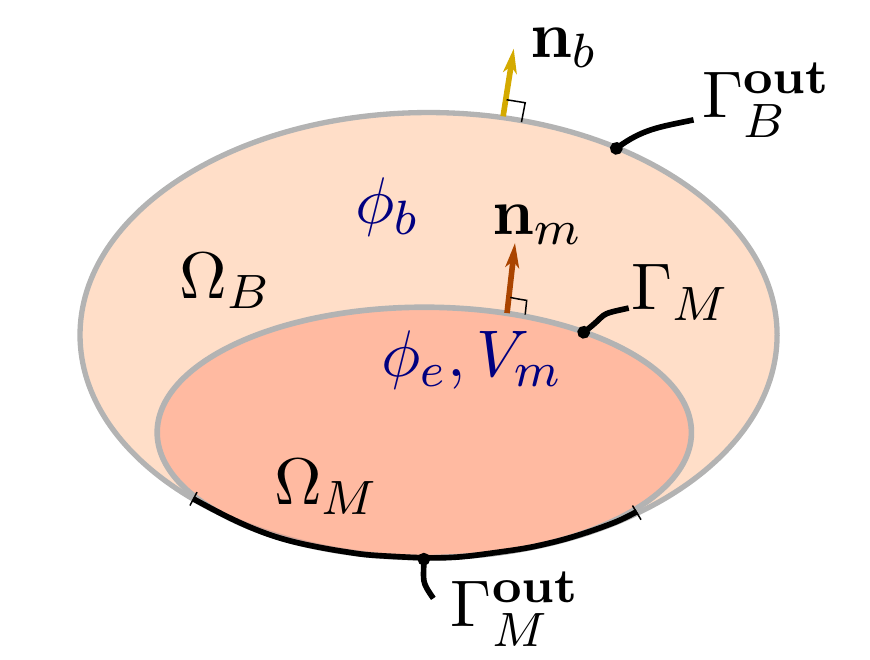
\includegraphics[width=50mm]{images/theory/computational_domains.png}
  \caption{Computational domains for the simulation of surface EMG. The body domain $\Omega_B$ and the muscle domain $\Omega_M$ share a part of their boundary, $\Gamma_M$, which has a normal vector $\bfn_m$. The outer boundary is composed of $\Gamma_B^\text{out}$ and $\Gamma_M^\text{out}$ and has the outward normal vector $\bfn_b$. }
  \label{fig:body_domain_visualization}
\end{figure}

The work of \cite{Mordhorst2015} proposes an isotropic conductivity $\bfsigma_b$ and a harmonic electric potential $\phi_b$ in the body domain $\Omega_B$:
\begin{align}\label{eq:body}
  \div \big(\bfsigma_b\,\grad (\phi_b)\big) = 0 \qquad \text{on } \Omega_B.
\end{align}

The electric potentials $\phi_e$ and $\phi_b$ of the neighboring domains $\Omega_M$ and $\Omega_B$ as well as the current densities are continuous on the shared boundary $\Gamma_M$. This is described by the following two coupling conditions:
\begin{subequations}\label{eq:body_domain_coupling}
  \begin{align}
    \phi_e &= \phi_b  \qquad &&\text{on } \Gamma_M, \label{eq:body_domain_bc1}   \\[4mm]
    \big(\bfsigma_e\, \grad( \phi_e)\big)\cdot \bfn_m &= \big(\bfsigma_b\, \grad(  \phi_b)\big)\cdot \bfn_m \qquad &&\text{on } \Gamma_M.\label{eq:body_domain_bc2}
  \end{align}
\end{subequations}
% 
On the outer boundary $\Gamma_B^\text{out}$, homogeneous Neumann boundary conditions are assumed:
\begin{align}% eq:body_domain_bc3
  \big(\bfsigma_b\, \grad( \phi_b)\big)\cdot \bfn_b &= 0 \qquad &&\text{on } \Gamma^\text{out}_B.\label{eq:body_domain_bc3}
\end{align}

The description of the body domain has to be combined either with the fiber based description in \cref{sec:monodomain_model} or the multi-domain description in \cref{sec:multidomain_model}. In the literature, this combination was mathematically described for the fiber based model in \cite{Mordhorst2015} and for the multidomain model in \cite{Klotz2020}. Correspondingly, additional boundary conditions either given by \cref{eq:monodomain_bc} or \cref{eq:multidomain_bc} are assumed: For the fiber based description, which uses the bidomain equation for volume conduction, the boundary conditions are:%
\begin{subequations}
\begin{align}
  \big(\bfsigma_i\,\grad(V_m)\big) \cdot \bfn_m &= -\big(\bfsigma_i\,\grad(\phi_e)\big)\cdot \bfn_m && \quad\text{on }∂\Omega_M=\Gamma_M \cup \Gamma_M^\text{out}, \label{eq:monodomain_fat_bc1}\\[4mm]
  \big(\bfsigma_e\,\grad(\phi_e)\big) \cdot \bfn_m &=0  && \quad\text{on }∂\Gamma_M^\text{out}. \label{eq:monodomain_fat_bc2}
\end{align}
\end{subequations}
%
For the multidomain description with fat layer, the boundary conditions are:
\begin{subequations}
\begin{align}
  \big(\bfsigma_i^k\,\grad(V_m^k)\big) \cdot \bfn_m &= -\big(\bfsigma_i^k\,\grad(\phi_e)\big)\cdot \bfn_m && \quad\text{on }∂\Omega_M=\Gamma_M \cup \Gamma_M^\text{out},  \label{eq:multidomain_fat_bc1}\\[4mm]
  \big(\bfsigma_e\,\grad(\phi_e)\big) \cdot \bfn_m &= 0 && \quad\text{on }∂\Gamma_M^\text{out}. \label{eq:multidomain_fat_bc2}
\end{align}
\end{subequations}
The first condition in \cref{eq:multidomain_fat_bc1} is enforced for all compartments $k=1,\dots,N_\text{MU}$.
%


% ----------


